\chapter{Introdução}


\section{Escopo}

Este exame de qualificação está estruturado em seis partes. A primeira parte
trata da apresentação do tema, com objetivos, justificativas e as estapas propostas no projeto de doutorado que foram concluídas, ou não. A segunda parte compõe um breve resumo sobre o paradigma da formação e evolução de bacias intracratônicas. A terceira parte apresenta a síntese do arcabouço geológico da Bacia do Parnaíba, mostrando um sumário sobre o preenchimento sedimentar, magmatismo e tectônica proposta em trabalhos anteriores. A quarta parte apresenta um artigo intitulado: \textit{"Deep crustal architecture of the Parnaíba basin of NE Brazil from receiver function analysis: Implications for basin subsidence"} que foi submetido para a The Geological Society Special Publications em março deste ano. A quinta e sexta partes propõem temas a serem estudados nos próximos semestre, como descontinuidades mantélicas de 410 km e 660 km através das funções do receptor e a tomografia de ruído sísmico ambiental, respectivamente.

\section{Objetivos}

Esta tese de doutorado tem por objetivo principal a caracterização estrutural, tanto crustal quanto mantélica, da Bacia do Parnaíba para buscar informações nesse arcabouço estrutural sobre os processos de formação e evolução na bacia. Com essa finalidade, foram elaborados objetivos secundários:

\begin{enumerate}
\item Determinação das estruturas crustais profundas na bacia atráves das estimativas pontuais de espessura crustal e razão Vp/Vs junto com perfis de velocidade de onda S obtidos na inversão conjunta entre funções do receptor e velocidades de ondas de superfície;

\item Imageamento das descontinuidades mantélicas de 410 km e 660 km, limites inferior e superior da Zona de Transição, para entender o papel da temperatura na evolução geológica da bacia;

\item Imagear o lineamento Transbrasiliano dentro da bacia atravéns da tomografia de ruído sísmico ambiental para entender o papel dessa mega-estrutura na formação e evolução da bacia;

\item Gerar subsídios para a proposição de um modelo de formação e evolução da Bacia do Parnaíba.

\end{enumerate}
\section{Justificativa}

A Bacia do Parnaíba, mesmo com um grande número de trabalhos realizados recentemente, ainda carece de muita informação sobre seu arcabouço estrutural crustal e mantélico. Esta bacia é tomada como paradigma para compreender o porquê de grandes áreas no interior de continentes, consideradas estáveis, em certos momentos de sua história passam por longos estágios de subsidência, ao longo dos quais são acumulados pacotes de rochas sedimentares com vários quilômetros de espessura associadas a manifestações vulcânicas episódicas. A maior parte do conhecimento sobre esta bacia é restrito a uma escala continental, como os estudos de \cite{feng_group_velocity_2004}, \cite{feng_upper_2007}, \cite{lloyd_moho_2010},\cite{van_der_meijde_gravity_2013},\cite{assumpcao_crustal_2013},\cite{assumpcao_models_2013},\cite{goutorbe_rayleigh_2015} e \cite{uieda_fast_2017}, e recentemente trabalhos regionais como os de \cite{de_castro_crustal_2014},\cite{daly_brasiliano_2014}, \cite{de_castro_geophysical_2016} e \cite{tozer_crustal_2017}. 

O presente trabalho encontra-se vinculado ao \textit{Parnaíba Basin Analysis Project}, uma parceria entre a BP Energy do Brasil  e várias universidades no Brasil e no Reino Unido, e tem com o objetivo melhorar o conhecimento sobre a origem e evolução dessa grande bacia cratônica no Norte-Nordeste do Brasil. Tal bacia é considerada uma fronteira exploratória, devido a descoberta de campos de gás natural durante a última década. Devido à sua grande dimensão, a maior parte do substrato sobre o qual a Bacia do Parnaíba se desenvolveu encontra-se encoberta, de forma que as informações disponíveis advêm majoritariamente de forma indireta. A análise conjunta de dados sismológicos, oriundos de sismos e de ruído ambiental, possibilita uma melhor resolução na observação de estruturas profundas e rasas no interior da bacia.

\section{Cronograma de Execução}

Após realizar as disciplinas propostas no projeto de Doutorado e ter um coeficiente de rendimento médio superior a 4, as únicas componentes curriculares obrigatórias pendentes são: Seminário de Pesquisa II, Exame de Qualificação, Exame de Proficiência em outra língua estrangueira diferente de inglês e Tese de Doutorado. Dos quais o Seminário de Pesquisa II e Exame de Qualificação eu já me encontro matriculado e devo cumprir no fim desse semestre. Restando apenas um exame de proficiência que devo cumprir no começo do próximo semestre e, por fim, a Defesa da Tese no final de 2018. 

\begin{figure}[!ht]
\begin{center}
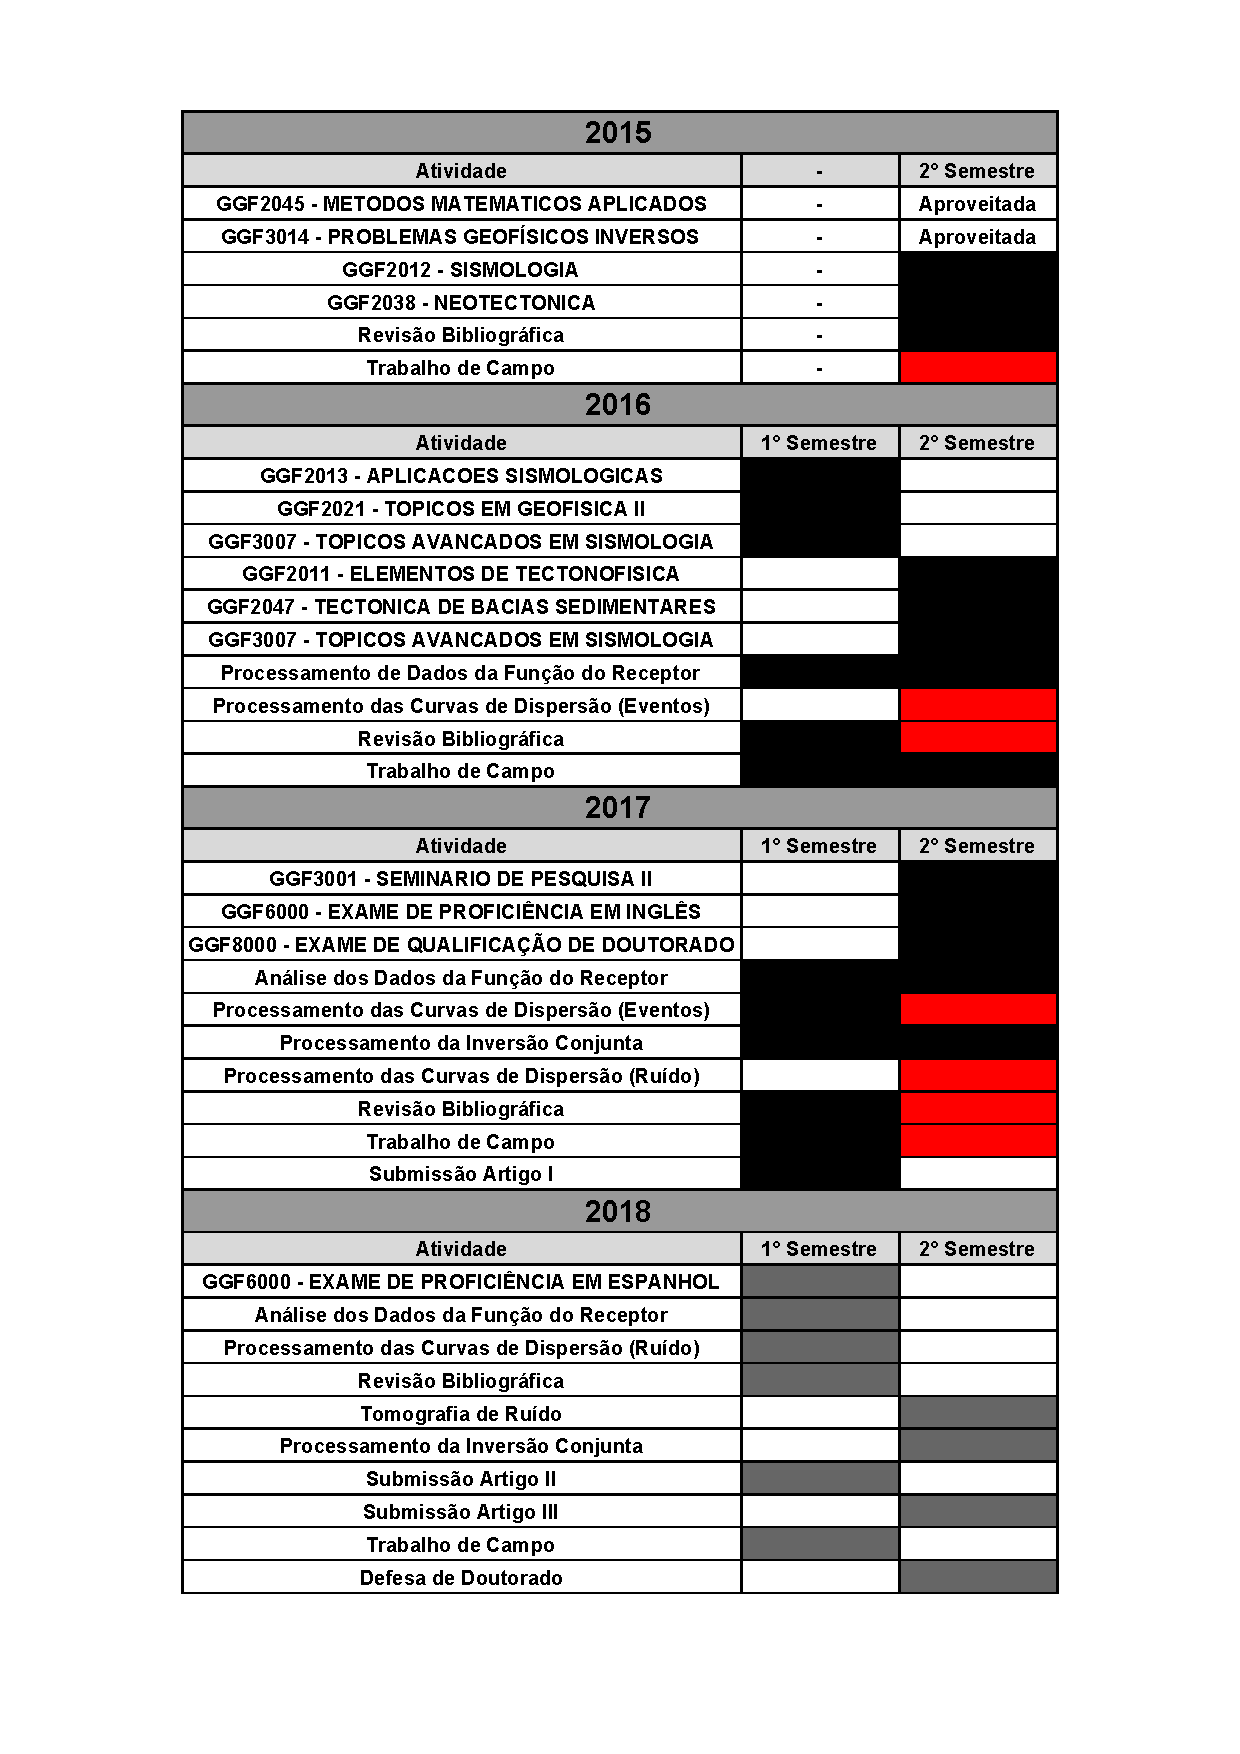
\includegraphics[width=1\textwidth]{Fig/cronograma.pdf}
\caption{Cronograma proposto no projeto de Doutorado. Preto - Etapas concluídas, Vermelho - estapas não concluídas na época prosposta, Cinza - Etapas futuras}
\label{mapa_sta_mantle}
\end{center}
\end{figure}